\documentclass[11pt,a4paper]{article}
\usepackage[margin=1in]{geometry}
\usepackage[T1]{fontenc}
\usepackage[utf8]{inputenc}
\usepackage{lmodern}
\usepackage{hyperref}
\usepackage{enumitem}
\usepackage{xurl}
\usepackage{tikz}
\usepackage{float}
\usetikzlibrary{arrows.meta, positioning, shapes.geometric}
\hypersetup{colorlinks=true,linkcolor=blue,urlcolor=blue}
\newcommand{\codepath}[1]{\path{#1}}
\tikzset{box/.style={rectangle,draw,rounded corners,align=center,inner sep=3pt,minimum width=36mm},line/.style={-Latex}}

\title{Phase-2 Deliverable: README (Scope Definition)}
\author{SIT Engine Architecture}
\date{\today}

\begin{document}
\maketitle

\section{Technical Description}
Phase-2 README defines scope, execution targets, adapter boundaries, and the workflow used to generate reproducible SIT artifacts. It is the architectural entrypoint for contributors adding new targets and replay checks.

\section{Implementation Fulfillment}
This deliverable is implemented in \codepath{Phase-2/README.md}. It references:
\begin{itemize}[leftmargin=*]
  \item orchestration: \codepath{Phase-2/riscvbench.py}, \codepath{Phase-2/cli.py},
  \item adapters: \codepath{Phase-2/adapters/},
  \item replay/validation scripts: \codepath{Phase-2/tests/run_golden_suite.py}, \codepath{Phase-2/tests/check_invariants.py},
  \item sweep tooling: \codepath{Phase-2/sweeps/run_param_sweep.py},
  \item cross-target smoke checks: \codepath{Phase-2/run_cross_target_suite.py}.
\end{itemize}
Cross-phase tracking currently exists in \codepath{Phase-1/docs/status/PHASE1_PHASE2_STATUS.md}.

\section{Design \& Architecture}
README acts as a control-plane specification:
\begin{itemize}[leftmargin=*]
  \item defines what is adapter logic versus engine logic,
  \item declares supported targets and runtime prerequisites,
  \item establishes reproducibility workflow (trace generation, replay, invariant checks, plots).
\end{itemize}
Dependencies: Adapter Contract, Golden Trace/Output policy, CI execution policy.

\subsection*{Function Flowchart}
\begin{figure}[H]
\centering
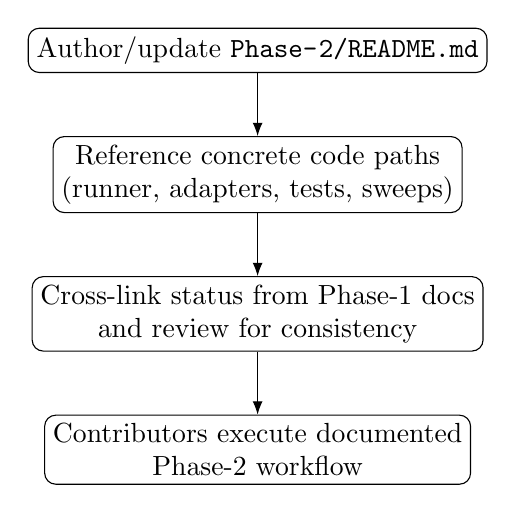
\begin{tikzpicture}[node distance=8mm and 12mm]
\node[box] (a) {Author/update \codepath{Phase-2/README.md}};
\node[box, below=of a] (b) {Reference concrete code paths\\(runner, adapters, tests, sweeps)};
\node[box, below=of b] (c) {Cross-link status from Phase-1 docs\\and review for consistency};
\node[box, below=of c] (d) {Contributors execute documented\\Phase-2 workflow};
\draw[line] (a) -- (b);
\draw[line] (b) -- (c);
\draw[line] (c) -- (d);
\end{tikzpicture}
\caption{Phase-2 README Flow}
\end{figure}

\end{document}
